\documentclass[a4paper]{article}
\setlength{\parskip}{\baselineskip}

\usepackage[a4paper,margin=25mm]{geometry}    % page layout
\usepackage{setspace} \onehalfspacing         % line spacing
\usepackage{amsfonts,amssymb,amsmath}         % useful math extensions
\usepackage{graphicx}                         % graphics import
\graphicspath{{../figs/}}
\pdfpageattr{/Group << /S /Transparency /I true /CS /DeviceRGB>>}
\usepackage[colorlinks=true, allcolors=black]{hyperref}
\usepackage{hhline}
\usepackage{subcaption}
% Change paragraph indentation
\setlength{\parskip}{10pt}
\setlength{\parindent}{0pt}
\usepackage[toc]{multitoc}
%\renewcommand*{\multicolumntoc}{2}
\setlength{\columnsep}{36pt}
\newcommand\numberthis{\addtocounter{equation}{1}\tag{\theequation}}
% topmatter
\title{\vspace{-50pt}\huge\bfseries Developing a Coarse-Grained Model
to Investigate Long-Term Climate Behaviour}
\author{Liam Wheen \\ Supervised by Dr O.\ Benjamin}

\date{\today}
\pagenumbering{gobble}

% main body
\begin{document}
\begin{titlepage}
\maketitle
\hrule
\vspace{-10pt}
\begin{abstract}
\noindent
This is the abstract.
\end{abstract}
\hrule
\end{titlepage}
%\vspace{20pt}
\newpage
\pagenumbering{gobble}
%\begin{spacing}{0.6}
\tableofcontents
%\end{spacing}
\newpage
\pagenumbering{arabic}
%\section{Introduction}
\section{Definitions}
\label{sec:definitions}
\begin{figure}
  \centering
  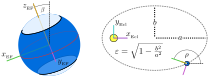
\includegraphics[width=0.8\linewidth]{orbital_params.pdf}
  \caption{Diagram of Earth from two perspectives, defining the three orbital
    parameters, obliquity $\beta$, eccentricity $\varepsilon$, and precession $\rho$. Also shown is the
    Earth centred Earth-fixed axes (EF), and the sun centred ecliptic axes
    (Ecl), with $z_{_{\mathrm{Ecl}}}$ pointing out of the page. Obliquity
    describes the tilt of Earth from vertical in the ecliptic frame.
    Eccentricity depends on the semi-major and semi-minor
    axes of Earth's orbit, $a$ and $b$ respectively. Precession describes the rotation of
  $x_{_{\mathrm{EF}}}$ about $z_{_{\mathrm{Ecl}}}$ from $x_{_{\mathrm{Ecl}}}$,
with all three vectors being Earth centred in this case.}
  \label{fig:orbital_params}
\end{figure}
Throughout this report, a number of parameters and reference frames will be
used. Here they will be defined and explained for future reference.

Figure \ref{fig:orbital_params} shows the 2 sets of axes that will be used to
describe orientation. Their origins will be located at either the centre of the
sun or the centre of Earth. \textit{The ecliptic frame}, shown here with its
origin at the sun, relates to the ecliptic plane, in which Earth's orbit lies.
The $x$-axis is parallel to the orbit's semi-major axis, whilst the $y$-axis is
parallel to the semi-minor axis of the orbit. Earth's position can be described
in the sun centred ecliptic frame using polar coordinates $\theta$ and $r$.
\textit{The Earth-fixed frame}, shown to be centred on Earth, rotates such that the
$x$-axis always points to coordinates $(0^\circ,0^\circ)$, the $y$-axis points
to $(0^\circ,90^\circ)$, and the $z$-axis points to the north pole. With these
axes centred on Earth, we can use spherical coordinates to describe a point on
Earth with the unit vector
\[
  \mathbf{u} = \begin{bmatrix}\cos\varphi\cos\gamma\\\cos\varphi\sin\gamma\\\sin\varphi\end{bmatrix}
\]
which points towards latitude $\varphi$ and longitude $\gamma$ on Earth.

For the Budyko model, and auxiliary models, we assume Earth to be homogeneous
over longitude. This allows us to ignore Earth's rotation
about its axis since longitude specific exposure to the sun is irrelevant, with
the focus being on the exposure at different latitudes. Hence we will treat the
Earth-fixed frame as aligning with the ecliptic frame, only rotating according
to the slow changing orbital parameters; obliquity and precession. These can be represented
in the Earth-fixed ecliptic frame with rotation matrices
\[
  U_{\beta} = \begin{bmatrix}\cos{\beta} & 0 & \sin{\beta}\\0 & 1 & 0\\-
  \sin{\beta} & 0 & \cos{\beta}\end{bmatrix},\quad\quad
  U_{\rho} = \begin{bmatrix}\cos{\rho} & - \sin{\rho} & 0\\\sin{\rho} &
  \cos{\rho} & 0\\0 & 0 & 1\end{bmatrix},
\]
for obliquity and precession respectively. $U_{\beta}$ acts first,
rotating about the ecliptic $y$-axis, followed by $U_{\rho}$, rotating
about the ecliptic $z$-axis.

\section{Milankovitch Cycles}
\begin{figure}[h]
  \centering
  \includegraphics[width=\linewidth]{orbital_param_time_series.pdf}
  \caption{Time series of the three orbital parameters over the past 3 million
  years. The data for which was produced by Laskar \cite{laskar2004}.}
  \label{fig:orbital_param_time_series}
\end{figure}

The Milankovitch cycles describe the periodic variation of the three orbital
parameters defined in Section \ref{sec:definitions}. That is obliquity,
precession, and eccentricity. The variation of these parameters over the past 3
million years can be seen in Figure \ref{fig:orbital_param_time_series}. This
data is calculated by Laskar \cite{laskar2004}, based on empirical data and
celestial mechanics.

As shown in Figure \ref{fig:orbital_params}, obliquity describes the tilt of
the Earth-fixed $z$-axis from the ecliptic $z$-axis. With a greater obliquity,
the poles are tilted closer to the ecliptic plane, and hence receive stronger
irradiance from the sun during their summer periods. This has the effect of
more evenly distributing insolation across Earth's latitudes, over a year
period. Taking the power spectrum of the time series data allows us to
determine its prominent frequencies, as shown in Figure \ref{fig:beta_power_spec}.
There is only one significant peak in the power spectrum, indicating that
obliquity maintains a reliable period of 41.1 thousand years (kyr). The amplitude
modulation visible in the obliquity plot of Figure \ref{fig:orbital_param_time_series} occurs with an
approximate period of 1 million years. This can be explained by the interaction
with the prominent frequency at 0.0243\,kyr$^{-1}$ and the slightly higher frequency of
0.0253\,kyr$^{-1}$, which has a far smaller amplitude. The sum of these two frequencies will
produce a beat frequency of $|0.0253-0.0243|=0.001$ which translates to a period
of $1/0.001=1000$\,kyr. However, because the higher of these two interfering frequencies is
of such a small amplitude, the resulting beat frequency does not show up on the
power spectrum.
\begin{figure}[h]
  \centering
  \includegraphics[width=0.9\linewidth]{beta_power_spec.pdf}
  \caption{Power spectrum for obliquity over the past 3 million years. A
    single peak occurs at 0.0243\,kyr$^{-1}$, meaning that obliquity oscillates
  with a period of 41.1\,kyr.}
  \label{fig:beta_power_spec}
\end{figure}

Axial Precession is the measure of pole rotation from the ecliptic $x$-axis. This is
an approximately constant clockwise rotation about the Earth centred ecliptic
$z$-axis. Precession governs the seasons on Earth. For example, the longest day
in the northern hemisphere will occur when the north pole's tilt aligns with
the sun. The current precession is illustrated in Figure \ref{fig:orbital_params},
with the northern summer solstice occurring a little before the aphelion of the
orbit. However as the north pole precesses clockwise, the summer solstice will
also move around the orbit in the clockwise direction, starting summer in the northern
hemisphere earlier.

The power spectrum for precession is shown in Figure \ref{fig:rho_power_spec},
with three significant frequencies identified. The weighted mean of these
frequencies is 0.0470, giving an average period of 21.3\,kyr for the last 3
million years. This period is only approximate, since the amplitude of these
frequencies is known to change depending on the timescale over which the data
is analysed. 
\begin{figure}[h]
  \centering
  \includegraphics[width=0.9\linewidth]{rho_power_spec.pdf}
  \caption{Power spectrum for precession over the past 3 million years. Three
  peaks are shown, occurring at 0.0423, 0.0447, and 0.0527\,kyr$^{-1}$, with their
corresponding periods shown in the legend.}
  \label{fig:rho_power_spec}
\end{figure}

The eccentricity of Earth's orbit is a measure of how elliptical it is, with 0
indicating a perfectly circular orbit. Earth's orbit has a maximum eccentricity
of around 0.06, which is close to circular when compared to planets such as
Mercury, with an eccentricity of 0.2. Despite this, we will see that
eccentricity still plays an important role in Earth's climatic behaviour.

The power spectrum for eccentricity, shown in Figure \ref{fig:ecc_power_spec},
reveals three prominent frequencies, with their equivalent periods shown in the
legend. The two higher frequencies, at 0.008\,kyr$^{-1}$ and
0.0103\,kyr$^{-1}$, are close enough to give a good approximation of the
prominent period, using a weighted mean this gives 109.1\,kyr. The lower
frequency peak at 0.0023\,kyr$^{-1}$ can again be explained by interference between the
other two frequencies, as we see the beat frequency is also $|0.0103 -
0.008|=0.0023$.
\begin{figure}[h]
  \centering
  \includegraphics[width=0.9\linewidth]{ecc_power_spec.pdf}
  \caption{Power spectrum for eccentricity over the past 3 million years. Three
    peaks are shown, occurring at 0.0023, 0.008, and 0.0103\,kyr$^{-1}$ with
  their corresponding periods shown in the legend.}
  \label{fig:ecc_power_spec}
\end{figure}

A commonly used method for measuring the change in insolation over a long
period involves measuring the average insolation at 65$^\circ$ north over the
summer solstice. This isolates the effect of the orbital parameters, avoiding
seasonal and latitudinal variations in insolation. The time series of
insolation at this point over the past 3 million years is shown in Figure
\ref{fig:N65_time_series}. This was generated with the daily insolation
simulation discussed in Section \ref{sec:insolation}, and verified with
McGehee's work \cite{insol_latlon}.
\begin{figure}
  \centering
  \includegraphics[width=0.9\linewidth]{N65_time_series.pdf}
  \caption{Insolation at 65$^\circ$ north during the summer solstice over the
  past 3 million years.}
  \label{fig:N65_time_series}
\end{figure}

The power spectrum for this data is shown in Figure \ref{fig:N65_power_spec}.
Here there are four prominent peaks, which can be seen to align with the power
spectrum peaks for obliquity and precession. The first peak corresponds to a
period of 41.1\,kyr, which is the period that obliquity varies over. The
remaining three periods are close to those of precession, ---

\begin{figure}
  \centering
  \includegraphics[width=0.9\linewidth]{N65_power_spec.pdf}
  \caption{Power spectrum for the daily insolation at 65$^\circ$ north during
    the summer solstice over the past 3 million years. Four peaks are shown,
    occurring at 0.0243, 0.042, 0.0443, 0.0523\,kyr$^{-1}$ with their
  corresponding periods shown in the legend.}
  \label{fig:N65_power_spec}
\end{figure}

\section{Budyko Model}
\label{sec:budyko}
The Budyko model is an energy balance model (EBM) that explores the positive
feedback effect of polar ice cap albedo. The increased reflectivity of polar
ice caps reduces the net energy that Earth can absorb from the sun across these
regions. If a sufficient amount of Earth's surface is covered in ice, 
global temperatures drop, and the polar ice caps advance towards the equator.
Conversely, if the ice caps only exist at very high latitudes, then the reduced
reflectivity will allow Earth to absorb more heat, and temperatures to rise,
leading the ice-line to recede further.

A number of assumptions are made in order for this EBM to work. Temperature
is modelled as varying only across latitude, reducing the domain of the
system from a spherical surface, to a 1-dimensional temperature profile. In
order to simplify integrals that span the latitudes, the
domain is described using $y = \sin\varphi$, where $\varphi$ is latitude.
To simplify the system further, the Earth is treated as an entirely water-based
planet. This allows for the differences in ground reflectivity to be ignored,
focusing only on the albedo of water and ice. The Earth is also modelled as
symmetric across the equator, allowing for only one half of the domain to be
considered, i.e. $y \in [0,1]$. This simplified domain is shown in Figure
\ref{fig:budyko_domain}. 

\begin{figure}
  \centering
  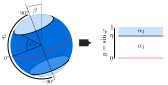
\includegraphics[width=0.7\linewidth]{budyko_domain.pdf}
  \caption{The change of domain used for the Budyko model, latitude $\varphi$
    becomes $y = \sin\varphi$ with only the northern hemisphere being
    considered. The ice line lies at latitude $\varphi_\eta$ and
    separates the water from the ice caps. This becomes $\eta$ in the new
    domain with range $[0,1]$. The albedo of sea is represented by
    $\alpha_1$, whilst the polar ice has albedo $\alpha_2$.}
  \label{fig:budyko_domain}
\end{figure}

The dynamical equation for temperature consists of three components. They
describe the flow of energy into, out of, and around Earth. The first of these
is incoming solar radiation, insolation, expressed by the term $Q_\varepsilon
s(y) (1-\alpha_\eta(y))$. The first component of this is the average yearly
insolation reaching Earth, $Q_\varepsilon$, which varies according to the
eccentricity of Earth's orbit, $\varepsilon$, such that $Q_\varepsilon =
Q_0/\sqrt{(1-\varepsilon^2)}$.

To calculate $Q_0$, we use the solar constant. This is attained
through satellite measurements and is the solar irradiance per unit area arriving
at Earth's atmosphere, one astronomical unit from the sun. This
irradiance is spread over the Earth's surface, $S = 4\pi r_\mathrm{E}^2$,
where $r_\mathrm{E}$ is the radius of the Earth. However Earth only
intercepts the sun's irradiance over an area equal to Earth's cross-section,
$\pi r_\mathrm{E}^2$. Hence the average yearly insolation is the solar
constant divided by 4. In similar work, this has been 343\,Wm$^{-2}$
\cite{widiasih2013,c_beta,insol_latlon} which is based on work by Tung from 2007
\cite{tung2007topics}. However, in this work Tung uses a solar constant of
1372\,Wm$^{-2}$, which is now considered significantly above the actual value.
Work done in 2011 by Kopp showed the current solar constant to be approximately
1361.5\,Wm$^{-2}$ \cite{solar_constant}, which would give
$Q_\varepsilon=340.375$\,Wm$^{-2}$, hence $Q_0 = Q_\varepsilon \sqrt{(1-\varepsilon^2)} =
340.327$\,Wm$^{-2}$ given the current value for $\varepsilon$, as shown in Table
\ref{tab:orbital_params}.
\begin{table}
  \centering
  \caption{Earth's orbital parameter values in the year 2020 along with their
  approximate ranges.}
\label{tab:orbital_params}
\begin{tabular}{c|c|c|c}
Parameter                    & Value  & Range               & Unit   \\ \hline\hline
Eccentricity ($\varepsilon$) & 0.0167 & 0.0005 - 0.0613     & None   \\ \hline
Obliquity ($\beta$)          & 0.4090 & 0.3814 - 0.4255     & Radians \\ \hline
Precession ($\rho$)          & 2.9101 & $-\pi$ -  $\pi$       & Radians
\end{tabular}
\end{table}
This insolation is then distributed
according to latitude. The full derivation of this even function is shown in
Section \ref{sec:insolation}. However, for this model we will use Widiasih's
approximation, which is within 2\% of the actual function, and is made up of
the even Legendre polynomials,
\[
  p_0(y) = 1,\quad\quad\quad\quad p_2(y) = \frac{1}{2}(3y^2-1),
\]
to give
\[
    s(y) = 1 + \frac{1}{2}c_\beta(3y^2-1),
\]
where $c_\beta = \frac{5}{16}(3\sin^2\beta - 2)$ and $\beta$ is obliquity
\cite{c_beta}. This approximation can be seen alongside the actual function in
Figure \ref{fig:yearly_ave_insol_present}. The final component of the
insolation term is $(1-\alpha_\eta(y))$, which describes the degree to which
heat is absorbed at a given latitude. This depends on the albedo of the
surface, which in this case is either water or ice. The albedo over our chosen domain
is therefore given as
\[
  \alpha_\eta(y) = \begin{cases} \alpha_1, & y<\eta\\
                                 \alpha_2, & y>\eta\\
                                 \frac{1}{2}(\alpha_1+\alpha_2), & y=\eta
                   \end{cases},
\]
where $\eta$ is the location of the ice line, whilst $\alpha_1=0.32$ and
$\alpha_2=0.62$ are established using satellite data \cite{tung2007topics}.
This results in less heat being absorbed over the area where ice is present
due to the increased reflectivity.

The next component of the equation is the outgoing infra-red radiation.
Although the energy flow occurring at the boundary between Earth and space is
complex, North performed linear regression on satellite data to
establish the net flow of long-wave radiation leaving Earth to the first order
\cite{linear_reradiation}. This gives
\[
  A+BT(y,t),
\]
where, for average cloud cover, $A=202.1$\,Wm$^{-2}$ and
$B=1.9$\,Wm$^{-2}\,^\circ$C$^{-1}$ with a correlation coefficient of 0.90.

The final component describes the transport of energy around Earth, from
the hot equator to the relatively cooler poles. The heat transport at a given
latitude is determined by the difference in temperature at this latitude and
the global average temperature, written as
\[
  C(\bar{T}(t)-T(y,t)),
\]
where
\[
  \bar{T}(t) = \int_0^1 T(y,t) \,\mathrm{d}y.
\]
By calculating the equilibrium temperature, $C$ can be chosen
such that the equilibrium matches current climatic conditions. Tung's work on
this yielded the relation $C=1.6B=3.04$\,Wm$^{-2}\,^\circ$C$^{-1}$ \cite{tung2007topics}.
Combining these components of heat flow gives the dynamical equation for temperature to be
\[
  R\frac{\partial T(y,t)}{\partial t} = \underbrace{Q_\varepsilon s(y) (1-\alpha_\eta(y))}_{\text{Insolation}}
  - \underbrace{(A+BT(y,t))}_{\text{Reradiation}}
  + \underbrace{C(\bar{T}(t)-T(y,t))}_{\text{Transport}}.
\]
This is known as an integro-differential equation, differing from a
conventional partial differential equation in that there is no derivative of
the spatial variable $y$. The only term that relates the temperature
at a given position to the rest of the system is $\bar{T}(t)=\int_0^1 T(y,t)
\,\mathrm{d}y$, which is the average global temperature.

To understand $R$, which governs the temperature's rate of change, we
inspect the units of the equation's terms. The insolation term
has units Wm$^{-2}$ from the $Q_\varepsilon$ component with the other two
components being dimensionless. The reradiation term describes radiation leaving
Earth per unit area, so again has units Wm$^{-2}$. Since $T$ is in $^\circ$C,
the units for $B$ are Wm$^{-2}$\,$^\circ$C$^{-1}$. $C$ is defined as $1.6B$ so
also has units Wm$^{-2}$\,$^\circ$C$^{-1}$, meaning the transport term is in
Wm$^{-2}$ as well. Since $\frac{\partial T(y,t)}{\partial t}$ will be in
$^\circ$C\,s$^{-1}$, the units for $R$ are J\,m$^{-2}$$^\circ$C$^{-1}$, which
equates to the heat capacity of Earth per unit area.

The value that $R$ takes will govern the rate at which the temperature profile
equilibrates. The heat capacity of water is approximately
4$\times10^3$J\,kg$^{-1}$$^\circ$C$^{-1}$ = 4$\times10^6$J\,m$^{-3}$$^\circ$C$^{-1}$,
using the relation that one cubic metre of water is 1000\,kg. With the assumption that Earth
is entirely water, that must be heated to a depth of 100\,m, we have that
\[
  R = 4\times10^8\mathrm{J\,m}^{-2}\,^\circ\mathrm{C}^{-1}.
\]
This is a very approximate value, however $R$ will not appear in
equilibrium solutions, relating only to the dynamic behaviour of the model.

A dynamic ice line was later introduced to the model by Widiasih
\cite{widiasih2013}, such that
\[
  S\frac{\mathrm{d}\eta(t)}{\mathrm{d}t} = T(\eta,t) - T_{\mathrm{ice}}
\]
where $T_{\mathrm{ice}}$ is an estimate for the critical temperature at which
an ice sheet can form.

\begin{table}[h]
  \centering
  \caption{Parameter values used for the Budyko model.}
  \label{tab:budyko_params}
\begin{tabular}{c|c|c|cl}
Parameter          & Value         & Unit        & Source &  \\ \hline\hline
$Q_0$              & 340.327       & Wm$^{-2}$   & Kopp \cite{solar_constant} \\\hline
$A$                & 202.1         & Wm$^{-2}$   & North \cite{linear_reradiation}  \\\hline
$B$                & 1.9           & Wm$^{-2}$\,$^\circ$C$^{-1}$ &  North \cite{linear_reradiation} \\\hline
$C$                & 3.04          & Wm$^{-2}$\,$^\circ$C$^{-1}$ &  Tung \cite{tung2007topics}\\\hline
$T_{\mathrm{ice}}$ & -10           & $^\circ$C   &  Tung \cite{tung2007topics}\\\hline
$\alpha_1$         & 0.32          & None        &  Tung \cite{tung2007topics}\\\hline
$\alpha_2$         & 0.63          & None        &  Tung \cite{tung2007topics}\\\hline
$R$                & $4\times10^8$ & Jm$^{-2}$\,$^\circ$C$^{-1}$ &  Widiasih \cite{c_beta}
\end{tabular}
\end{table}
\begin{figure}
\centering
\begin{subfigure}{.4\textwidth}
  \centering
  \includegraphics[width=\linewidth]{demo_budyko_0.pdf}
  \vspace{-23pt}
  \caption{0 Years}
\end{subfigure}%
\vspace{10pt}
\begin{subfigure}{.4\textwidth}
  \centering
  \includegraphics[width=\linewidth]{demo_budyko_1.pdf}
  \vspace{-23pt}
  \caption{10 Years}
\end{subfigure}
\vspace{10pt}
\begin{subfigure}{.4\textwidth}
  \centering
  \includegraphics[width=\linewidth]{demo_budyko_2.pdf}
  \vspace{-23pt}
  \caption{3000 Years}
\end{subfigure}%
\begin{subfigure}{.4\textwidth}
  \centering
  \includegraphics[width=\linewidth]{demo_budyko_3.pdf}
  \vspace{-23pt}
  \caption{10\,000 Years}
\end{subfigure}
\caption{Snapshots of a Budyko simulation starting with 0$^\circ$C at all
latitudes and the ice line at $\eta=0.5$. The model parameters used are shown
in Table \ref{tab:budyko_params} whilst the initial orbital parameters are in
Table \ref{tab:orbital_params}. We first see the temperature profile
equilibrate within 10 years. The ice line then recedes 
towards the stable equilibrium point at $y=0.9544$, getting within 3\% of this
value after 10\,000 years.}
\label{fig:budyko_demo}
\end{figure}
[Need to justify the 340, mention how Tung is using too large solar constant]
[Here discuss the introduction of the dynamic iceline from widiasih, the
  dynamics of the model, the equilibrium points, the stability, how this
  doesn't get effected by the milankovitch params much at all, the lack of any
  oscillation (which I believe would be impossible anyway given the equations
  formulation), the slow and fast dynamics of the temp and iceline
respectively (as shown in the figure).]
[Also introduce Milankovitch properly and how each orbital parameter is defined
(especially precession). Maybe move Table of orbital params up to milankovitch
section]
\section{Insolation}
\label{sec:insolation}
Insolation is solar irradiance integrated over time, however we are usually
interested in the average insolation over a given time period, hence the units
for both irradiance and average insolation are Wm$^{-2}$. We will first look at
average daily insolation to see how this varies throughout a year, then a
yearly average will be used to investigate long-term changes to insolation
across different latitudes. We can then compare this with the approximations
used in the Budyko model to see how they differ. All simulations that depend on
the Milankovitch cycles take this data from Laskar \cite{laskar2004}.

To model the average insolation over a chosen period, we first express
the irradiance arriving at a given point on Earth, in terms of the orbital
parameters, latitude, and longitude. For this we will use an Earth centred
Earth-fixed frame.

Firstly, we express the total irradiance arriving at Earth's atmosphere. This
is calculated using the inverse square law, distributing the total solar
output $K$ over the surface area of an imagined sphere with a radius
equal to Earth's distance from the sun. This gives
\[
  \frac{K}{4\pi r^2}\,\,\mathrm{Wm^{-2}}.
\]

Recall that a point on Earth, given by ($\varphi,\gamma$), can be expressed
with the unit vector
\[
  \mathbf{u} = \begin{bmatrix}\cos\varphi\cos\gamma\\\cos\varphi\sin\gamma\\\sin\varphi\end{bmatrix}
\]
The irradiance at ($\varphi,\gamma$) is proportional to the cosine of the angle
between $\mathbf{u}$ and the vector that points from Earth to the sun,
$\mathbf{n}$. This vector uses $\theta$, Earth's angle around the sun in
ecliptic polar coordinates, expressed in the Earth centred Earth-fixed frame as
\[
  \mathbf{n} = \left(U_{\rho}U_{\beta}\right)^{-1}\begin{bmatrix}-\cos\theta\\-\sin\theta\\0\end{bmatrix} = 
  \begin{bmatrix}-\cos{\beta} \cos(\rho - \theta)\\
  \sin(\rho - \theta)\\-\sin{\beta} \cos(\rho -\theta)\end{bmatrix}.
\]
Multiplying the scalar product of these two unit vectors by the irradiance at
the atmosphere gives
\[
  \begin{split}
    I(r,\theta,\beta,\rho,\varphi,\gamma) &= \frac{K}{4\pi
    r^2}\,\mathbf{u}^\top\mathbf{n}\\
  &=\frac{K}{4\pi r^2}
  \begin{bmatrix}\cos\varphi\cos\gamma\\\cos\varphi\sin\gamma\\\sin\varphi\end{bmatrix}^\top
  \begin{bmatrix}-\cos{\beta} \cos(\rho - \theta)\\
  \sin(\rho - \theta)\\-\sin{\beta} \cos(\rho -\theta)\end{bmatrix}\\
  &= \frac{K}{4\pi r^2}[(\sin{\gamma}\sin{(\rho - \theta)}-\cos{\beta} \cos{\gamma}
    \cos{(\rho-\theta)})\cos{\varphi}
  -\sin{\beta}\sin{\varphi} \cos{(\rho -\theta)}].
\end{split}
\]

Note this expression is only valid for positive values, since the irradiance
value for the dark side of Earth will be negative, when it should be 0. To
calculate the average daily insolation, we can treat the orbital parameters as
constant and integrate with respect to longitude $\gamma$ over the range
$[0,2\pi]$. However, since this expression is only valid for positive values,
we must either augment our expression for irradiance $I$ to be the piecewise
function Max$(0,I)$, or define the limits such that we only integrate over the
range of longitudes that receive sunlight. Through simulation, the former
approach was found to be far more computationally costly as the piecewise
needed evaluating at every step of the integration, whereas the piecewise
limits only need to be calculated once. 

To find these limits in terms of the orbital parameters, we consider a plane
passing through the origin, separating the light and dark hemispheres of Earth,
rotating so that its normal vector always points towards the sun. The plane can
therefore be expressed as
\[
  ax+by+cz=0,
\]
where $a$, $b$, and $c$ are the components of $\mathbf{n}$.

Next consider a circle of constant latitude $\varphi$, lying parallel to the
$x$-$y$ plane such that
\[
  x^2+y^2 = \cos^2\varphi.
\]
This derivation is using a unit sphere for convenience since longitude is
invariant with size. The intersections of this circle with the plane
separating day and night indicate the limits over which integration should be
performed for the given latitude and orbital parameters. An example of this can
be seen in Figure \ref{fig:circ_plane_intercept}.
\begin{figure}
  \centering
  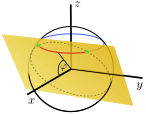
\includegraphics[width=0.6\linewidth]{circ_plane_intercept.pdf}
  \caption{Diagram showing the day-night plane (yellow) that passes through the
    origin at Earth's centre and rotates to face the sun, and the circle of
    constant latitude $\varphi$. The points where the circle intersects the plane
    (green) indicate the range of longitudes for which sunlight will reach Earth
  at latitude $\varphi$ (red) whilst longitudes on the opposite side of the
plane (blue) are in darkness so receive no insolation.}
  \label{fig:circ_plane_intercept}
\end{figure}

Using the final condition that 
\[
  z = \sin\varphi,
\]
we find the two intersection points to be
\[
  \boldsymbol{\mu}_{0,1}=\frac{1}{a^2 + b^2}\begin{bmatrix}- a c \sin{\varphi}\mp b
    \sqrt{\left(a^2+b^2\right) \cos^2{\varphi}- c^2 \sin^2{\varphi}}\\
  - b c \sin{\varphi}\pm a \sqrt{\left(a^2+b^2\right) \cos^2{\varphi}
  - c^2 \sin^2{\varphi}}\\
(a^2 + b^2)\sin{\varphi}\end{bmatrix}.\numberthis
\label{eq:integration_limits}
\]

Looking at (\ref{eq:integration_limits}), we see there are two real
solutions when the discriminant, 
\[
  \left(a^2+b^2\right) \cos^2{\varphi} - c^2 \sin^2{\varphi} = \Delta,
\]
is positive.

If $\Delta \le 0$, then there is either no intersection between the circle
and the plane, or only one. Hence the entire circle of latitude $\varphi$ will lie
on the dark, or light, side of the plane.

To determine which side it is, we return to the scalar product
$\mathbf{u}^\top\mathbf{n}$ where $\mathbf{u}$ will point to some part of the
circle, for simplicity we choose $(\varphi,0)$. If no intersection has
occurred and $\mathbf{u}^\top\mathbf{n}$ is positive, then this point and the
entirety of the circle lies within sunlight, whilst a negative product 
corresponds to darkness. This is written as
\[
  \mathbf{u}^\top\mathbf{n}\,\bigr|_{\gamma=0} = -\cos\left(\beta - \varphi
  \right) \cos\left(\rho - \theta \right).
\]

In the rare case that this is exactly equal to 0, a different point on the
circle would be chosen.

The intersection points, $\boldsymbol{\mu}_0$ and $\boldsymbol{\mu}_1$, are
currently expressed in Cartesian coordinates. For the corresponding longitudes
we use the general relation $\gamma = \arctan\left(\frac{y}{x}\right)$. We can now
express the longitudinal limits in piecewise form as
\[\gamma_0 = \begin{cases}
    \arctan\left(\frac{\mu_{0y}}{\mu_{0x}}\right), & \Delta>0\\
    0, & \Delta\le 0
  \end{cases},
  \quad\quad\quad
  \gamma_1 = \begin{cases}
    \arctan\left(\frac{\mu_{1y}}{\mu_{1x}}\right), & \Delta>0\\
    2\pi, &\Delta\le 0 \land\mathbf{u}^\top\mathbf{n}\,\bigr|_{\gamma=0}> 0\\
    0, &\Delta\le 0 \land\mathbf{u}^\top\mathbf{n}\,\bigr|_{\gamma=0}< 0
  \end{cases},
\]
where the limits become either $[0,2\pi]$ or $[0,0]$ if the given latitude lies
entirely in day or night respectively.

The calculation for daily average insolation is therefore
\[\begin{aligned}
  Q_{\mathrm{day}} &= \frac{1}{2\pi} \frac{K}{4\pi
  r^2}\int_{\gamma_0}^{\gamma_1} (\sin{\gamma}\sin{(\rho - \theta)}-\cos{\beta} \cos{\gamma}
    \cos{(\rho-\theta)})\cos{\varphi} -\sin{\beta}\sin{\varphi} \cos{(\rho
    -\theta)}\,\mathrm{d}\gamma\\ 
  &=\frac{K}{8\pi^2r^2}[(\gamma_{0} - \gamma_{1}) \sin{\beta}
  \sin{\varphi} \cos{\left(\rho - \theta \right)} +
  (\sin{\gamma_{0}} \cos{\beta}
  \cos{\left(\rho - \theta \right)} - \sin{\gamma_{1}} \cos{\beta} \cos{\left(\rho - \theta \right)}\\
&\quad\quad\quad\quad\quad\quad + \sin{\left(\rho - \theta \right)} 
\cos{\gamma_{0}} - \sin{\left(\rho - \theta
\right)} \cos{\gamma_{1}} ) \cos{\varphi}].
\end{aligned}
\]

Using this expression, Figure \ref{fig:daily_ave_insol_all_lats} shows
how insolation varies over a year period, at each latitude, using current orbital
parameters. The second plot in this figure shows the same year, but with
eccentricity increased to 0.06, approximately the maximum eccentricity
of Earth's orbit. The third plot shows the difference between the two cases,
where a positive value corresponds to more insolation in the second plot.
\begin{figure}
  \hspace{-40pt}
  \includegraphics[width=1.2\linewidth]{both_daily_ave_insolation_all_lats.pdf}
  \caption{Contours showing the daily average insolation arriving at the
    atmosphere for different latitudes over a year period. The left plot is
    based on current orbital parameters, from Table \ref{tab:orbital_params}.
    In the second plot, eccentricity is increased to 0.06, approximately the
    maximum for Earth's orbit. The third plot shows how these two cases differ,
    where a positive value corresponds to more insolation in the second plot.}
  \label{fig:daily_ave_insol_all_lats}
\end{figure}

The summer solstice in the northern hemisphere currently occurs 13 days before
the aphelion of Earth's orbit, meaning Earth is almost the farthest it can be
from the sun. Conversely, summer in the southern hemisphere begins 170 days after the
aphelion, when Earth is almost the nearest it can be to the sun. Since the
irradiance that reaches Earth is proportional to $1/r^2$, where $r$ is the
distance from Earth to the sun, we see more insolation in the southern
hemisphere over its summer solstice than in the northern hemisphere's summer
solstice. The difference plot in Figure \ref{fig:daily_ave_insol_all_lats}
confirms this. Showing that greater eccentricity leads to a greater difference
between maximum insolation values in the hemispheres.

Kepler's second law states
\[
  \frac{\mathrm{d}\theta}{\mathrm{d}t} = \frac{2\pi a b}{Pr^2},
\]
where $P$ is the year period, and $a$ and $b$
are the semi-major and semi-minor axes respectively. On the scale of a year,
these can be considered constant, meaning Earth's angular speed
around the sun is proportional to $1/r^2$.

As eccentricity increases and the distance between the perihelion and the sun
decreases, the angular speed around this region will increase. This is the
cause of the 2 spikes at either pole in the difference plot of Figure
\ref{fig:daily_ave_insol_all_lats}. These indicate where the more eccentric
orbit has traversed the angular range around the perihelion faster than our
actual orbit. This results in the summer period in the southern hemisphere
lasting less time, becoming comparatively cooler either side of the warmest 100
days. Whilst at the same time in the northern hemisphere, winter is shorter,
leading to comparatively warmer periods either side of the coldest 100 days.

Although eccentricity appears to effect the insolation in each hemisphere
differently, we will see later that they still receive the same total insolation over
a year period.

We will now express the average yearly insolation as a function of orbital
parameters, using work by McGehee and Lehman \cite{insol_latlon}. 
Recall the expression for irradiance at a given point is
\[\begin{aligned}
  I(r,\theta,\beta,\rho,\varphi,\gamma) &= \frac{K}{4\pi r^2}\mathbf{u}^\top\mathbf{n}\\
    &= \frac{K}{4\pi
    r^2}\begin{bmatrix}\cos\varphi\cos\gamma\\\cos\varphi\sin\gamma\\\sin\varphi\end{bmatrix}^\top
    U_{\beta}^{-1}U_{\rho}^{-1}\begin{bmatrix}-\cos\theta\\-\sin\theta\\0\end{bmatrix},
  \end{aligned}
\]
which is only valid for positive values of $I$.

It will be useful to define 
\[
  \begin{bmatrix}\cos\varphi\cos\gamma\\\cos\varphi\sin\gamma\\\sin\varphi\end{bmatrix}^\top
  U_{\beta}^{-1} = \begin{bmatrix}\sin{\beta} \sin{\varphi } + \cos{\beta}
  \cos{\gamma} \cos{\varphi}\\\sin{\gamma} \cos{\varphi }\\\cos{\beta }\sin{\varphi} - \sin{\beta} \cos{\gamma}
\cos{\varphi} \end{bmatrix}^\top =
  \begin{bmatrix}\cos\hat{\varphi}\cos\hat{\gamma}\\\cos\hat{\varphi}\sin\hat{\gamma}\\\sin\hat{\varphi}\end{bmatrix}^\top,\numberthis
  \label{eq:u_hat_definition}
\]
where $\hat{\varphi}$ and $\hat{\gamma}$ can be visualised as the latitude and
longitude measured not from the north pole, but from the $z$-axis in the
Earth centred ecliptic frame. The irradiance at a given point can therefore be written as
\[
  I = \frac{K}{4\pi r^2}\begin{bmatrix}\cos\hat{\varphi}\cos\hat{\gamma}\\
  \cos\hat{\varphi}\sin\hat{\gamma}\\\sin\hat{\varphi}\end{bmatrix}^\top 
  U_{\rho}^{-1}\begin{bmatrix} -\cos{\theta}\\-\sin{\theta}\\0\end{bmatrix} 
  = -\frac{K}{4\pi r^2} \cos\hat{\varphi}\cos{\left(\hat{\gamma} + \rho -
  \theta \right)}.
\]
Treating the orbital parameters as fixed, the average insolation over a year
period $P$ is given as
\[
  Q = \frac{1}{P}\int_0^P\frac{-K}{4\pi r^2}
  \cos\hat{\varphi}\cos{\left(\hat{\gamma} + \rho - \theta
  \right)}\,\mathrm{d}t,\numberthis
  \label{eq:yearly_insol_integral_dt}
\]
however, since $r$ and $\theta$ have a non-linear dependence on time, we shall
use $\theta$ as the variable of integration. Returning to Kepler's second law,
we know that
\[
  \frac{\mathrm{d}t}{\mathrm{d}\theta} = \frac{Pr^2}{2\pi ab},
\]
where $a$ and $b$ are the semi-major and semi-minor axes of Earth's orbit
respectively.

Substituting $\theta$ for $t$ in (\ref{eq:yearly_insol_integral_dt}) now
gives
\begin{align}
    Q &=\frac{1}{P}\int_0^{2\pi}\frac{-K}{4\pi r^2}
    \cos\hat{\varphi}\cos{\left(\hat{\gamma} + \rho - \theta \right)}
    \frac{Pr^2}{2\pi a b}\,\mathrm{d}\theta\nonumber\\ 
    &=\frac{K\cos\hat{\varphi}}{8\pi^2
    a b}\int_0^{2\pi}-\cos{\left(\hat{\gamma} + \rho - \theta \right)}
    \,\mathrm{d}\theta.\label{eq:yearly_insol}
\end{align}
Since the expression for $I$ is only valid for positive values, the integral in
(\ref{eq:yearly_insol}) is equivalent to the positive area under $\cos\theta$ 
from 0 to 2$\pi$, which gives 2. The average yearly insolation at a given point is therefore
\[
  Q = \frac{K\cos\hat{\varphi}}{4\pi^2 a b}.
\]
Note that this is independent of precession, meaning that over a year, its
effect on insolation is cancelled out at all latitudes.

In order to express average yearly insolation over a latitude,
we must average $Q$ over longitude, $\gamma$. It will be of more use to
express this in the Earth-fixed frame, using the conventional latitude values.
For this we refer to (\ref{eq:u_hat_definition}), which defines
\[
  \sin{\hat{\varphi}} = \cos{\beta}\sin{\varphi} -
  \sin{\beta}\cos{\gamma}\cos{\varphi},
\]
hence
\[
  Q = \frac{K\sqrt{1 -\left( \cos{\beta}\sin{\varphi} -
  \sin{\beta}\cos{\gamma}\cos{\varphi}\right)^2}}{4\pi^2 a b}.
\]

We now average this over longitude to get
\[
  \frac{K}{4\pi^2 a b}\frac{1}{2\pi} \int_0^{2\pi}\sqrt{1 -\left( \cos{\beta}\sin{\varphi} -
  \sin{\beta}\cos{\gamma}\cos{\varphi}\right)^2}\,\mathrm{d}\gamma.
\]

In order to express this purely as a function of orbital parameters and
latitude, we use the relation $b = a\sqrt{1-\varepsilon^2}$, where
$\varepsilon$ is orbital eccentricity. Laskar found that $a$ remains
essentially constant, regardless of orbital parameters \cite{laskar2004}. This
means that the average yearly insolation for a given latitude only depends on
$\varepsilon$ and $\beta$, such that
\[
  Q_{\mathrm{year}}(\varepsilon,\beta,\varphi) = \frac{K}{8\pi^3 a^2
  \sqrt{1-\varepsilon^2}}\int_0^{2\pi}\sqrt{1 -\left( \cos{\beta}\sin{\varphi} -
  \sin{\beta}\cos{\gamma}\cos{\varphi}\right)^2}\,\mathrm{d}\gamma.
\]

To compare this to the insolation term in the Budyko model, we make
the substitution $y = \sin\varphi$, giving
\[
  Q_{\mathrm{year}}(\varepsilon,\beta,y) = \frac{K}{8\pi^3 a^2
  \sqrt{1-\varepsilon^2}}\int_0^{2\pi}\sqrt{1 -\left( y\cos{\beta} -
  \sqrt{1-y^2}\sin{\beta}\cos{\gamma}\right)^2}\,\mathrm{d}\gamma.\numberthis
  \label{eq:q_year_budyko}
\]

Omitting the albedo component, insolation in the Budyko model is given by
$Q(\varepsilon)s(\beta,y)$, where 
\[
  Q(\varepsilon) = \frac{Q_0}{\sqrt{1-\varepsilon^2}},\quad\quad\quad 
  s(\beta,y) = 1 + \frac{1}{2}c(\beta)(3y^2-1).
\]
The $Q(\varepsilon)$ term represents the average yearly insolation, whilst
$s(\beta,y)$ distributes this according to latitude and obliquity. The integral
of $s(\beta,y)$ in the range $y\in[0,1]$ is unity, satisfying that the global average
insolation will be $Q(\varepsilon)$.

The solar constant is the irradiance per unit area at Earth's atmosphere,
1 astronomical unit (AU) from the sun. Recall that $Q_0$ is found by
dividing the solar constant by 4, due to the ratio of the area that intercepts
the sun's rays to Earth's total surface area. Since 1\,AU is defined as the
semi-major axis of Earth's orbit, the solar constant can be expressed as
$\frac{K}{4\pi a^2}$, where $K$ is the total solar output and $a$ is the
semi-major axis. We can therefore write
\[
  Q(\varepsilon) =\frac{Q_0}{\sqrt{1-\varepsilon^2}}= \frac{K}{16\pi a^2 \sqrt{1-\varepsilon^2}}.
\]
By substituting this into (\ref{eq:q_year_budyko}), we see that
$s(\beta,y)$ is approximating the function
\[
  \frac{2}{\pi^2}\int_0^{2\pi}\sqrt{1 -\left( y\cos{\beta} -
  \sqrt{1-y^2}\sin{\beta}\cos{\gamma}\right)^2}\,\mathrm{d}\gamma,
\]
which also equates to 1 when integrated over the range $y\in[0,1]$.
This function for insolation, along with the Budyko approximation, can be see in Figure
\ref{fig:yearly_ave_insol_present}. 
\begin{figure}
  \centering
  \includegraphics[width=0.5\linewidth]{yearly_average_insol_present.pdf}
  \caption{The average yearly insolation, $Q_{\mathrm{year}}$, for current orbital parameters, as
    shown in Table \ref{tab:orbital_params}. The dashed line shows the
    approximation for yearly insolation used in the Budyko model as discussed
  in Section \ref{sec:budyko}. The shape of $Q_\varepsilon s(y)$ has been warped here
to fit the domain of $\varphi$, as opposed to $y=\sin\varphi$.}
  \label{fig:yearly_ave_insol_present}
\end{figure}
\begin{figure}
  \centering
  \includegraphics[width=0.9\linewidth]{beta_eps_effect.pdf}
  \caption{Plots showing the effect of obliquity (left) and eccentricity
    (right) on the average yearly insolation across latitudes. Unless stated,
  parameter values are $\beta = 0.4091$ and $\varepsilon = 0.0167$. The
parameters are given values beyond their actual ranges to demonstrate their
effect. Their actual ranges are give in Table \ref{tab:orbital_params}.}
  \label{fig:beta_eps_effect}
\end{figure}

By breaking the insolation expression into two terms, $Q(\varepsilon)$ and
$s(\beta,y)$, the effect of obliquity and eccentricity on yearly insolation can
be isolated. This is shown in Figure \ref{fig:beta_eps_effect}, where each plot
varies one of the two orbital parameters. Since $\varepsilon$ only appears in the component for global
average insolation, we see that eccentricity will only scale the insolation
curve. Conversely, $\beta$ is only present in the function $s(y)$, which
distributes the insolation according to latitude and always integrates to
1 over the range $y\in[0,1]$. We therefore see the shape of the curve varying
with $\beta$, but not the area underneath it.

We can see how these orbital parameters take effect in Figure
\ref{fig:yearly_ave_insol_all_lats}, showing the change in average yearly
insolation, over the past 150 thousand years. 
\begin{figure}
  \centering
  \includegraphics[width=0.6\linewidth]{yearly_average_insol_150kN.pdf}
  \caption{Contour showing the difference in yearly average insolation from the
  average insolation over the 150k year period at each latitude. At the
  top and bottom are eccentricity $\varepsilon$ and obliquity $\beta$, the two
orbital parameters that govern the yearly average insolation.}
  \label{fig:yearly_ave_insol_all_lats}
\end{figure}

When obliquity is greater, the equator aligns less with the ecliptic plane, absorbing
less insolation over the year. However the poles point closer towards the sun
for one half of the year, and still receive no insolation during the other
half. This increases yearly insolation around the poles and decreases it around the
equator, as can be see in Figure \ref{fig:yearly_ave_insol_all_lats}. More
subtly, as eccentricity drops to lower values at around $-80$\,k years ago, we
see the overall global insolation lowering slightly from red to blue. 

In all of the plots shown, we can see that the functions are even about the
equator, meaning yearly insolation is always equally distributed between the
two hemispheres. Kepler's second law tells us that the angular speed of Earth
around the sun is proportional to $1/r^2$, meaning it will take longer for
Earth to traverse some orbital range $\psi$ around the aphelion of its orbit,
where $r$ takes the greatest value, compared to the perihelion.

Recall that the irradiance is also proportional to $1/r^2$. Hence, for $\psi$
at the aphelion, the increased duration is counteracted by the reduced
irradiance, whilst the greater irradiance at the perihelion is experienced for
proportionally less time. Applying this to an arbitrary latitude, we will see
how this results in a symmetric insolation curve when averaged over a whole
orbit.

To express insolation over the orbital range $\psi$, we integrate over
$\theta$. We again treat Earth as non-rotating, instead integrating over
longitude, $\gamma$. It is useful to separate our expression for irradiance at
a given point into two components, such that
\[
  I(r,\theta,\beta,\rho,\varphi,\gamma) =
  \frac{K}{4\pi r^2}S(\theta,\beta,\rho,\varphi,\gamma),
\]
where 
\[
  S(\theta,\beta,\rho,\varphi,\gamma) = (\sin{\gamma}\sin{(\rho -
  \theta)}-\cos{\beta} \cos{\gamma} \cos{(\rho-\theta)})\cos{\varphi}
  -\sin{\beta}\sin{\varphi} \cos{(\rho -\theta)}.
\]
We first measure the insolation over $\psi$ on the aphelion side
of the orbit, which occurs at angle $\theta_{\mathrm{A}}$. This is measured at
latitude $\varphi$, which we will choose to be in the northern hemisphere. This
gives
\[
  Q_{\mathrm{A}} = \int_{t(\theta_{\mathrm{A}}-\frac{\psi}{2})}^{t(\theta_{\mathrm{A}}+\frac{\psi}{2})}
  \int_{\gamma_1^{\mathrm{N}}}^{\gamma_2^{\mathrm{N}}}
  \frac{K}{4\pi r^2} S(\theta,\beta,\rho,\varphi,\gamma)\, \mathrm{d}\gamma\,\mathrm{d}t,
\]
where $t(\theta)$ is the time that corresponds to orbital angle $\theta$. Note
that the longitudinal limits also depend on $\theta, \beta, \rho$, and
$\varphi$, which vary so as to only span the positive range of $S$. This is shown by the red
regions in Figure \ref{fig:gamma_limits}.

Changing the variable of integration to $\theta$, we obtain
\begin{align*}
    Q_{\mathrm{A}} &= \int_{\theta_{\mathrm{A}}-\frac{\psi}{2}}^{\theta_{\mathrm{A}}+\frac{\psi}{2}}
    \int_{\gamma_1^{\mathrm{N}}}^{\gamma_2^{\mathrm{N}}}
  \frac{K}{4\pi r^2}S(\theta,\beta,\rho,\varphi,\gamma)\,\mathrm{d}\gamma\,\frac{\mathrm{d}t}{\mathrm{d}\theta}\,\mathrm{d}\theta\\
  &=\int_{\theta_{\mathrm{A}}-\frac{\psi}{2}}^{\theta_{\mathrm{A}}+\frac{\psi}{2}}\int_{\gamma_1^{\mathrm{N}}}^{\gamma_2^{\mathrm{N}}}
  \frac{K}{4\pi r^2}\frac{Pr^2}{2\pi a b}S(\theta,\beta,\rho,\varphi,\gamma)\, \mathrm{d}\gamma\,\mathrm{d}\theta\\
  &=\frac{KP}{8\pi^2 a
  b}\int_{\theta_{\mathrm{A}}-\frac{\psi}{2}}^{\theta_{\mathrm{A}}+\frac{\psi}{2}}
  \int_{\gamma_1^{\mathrm{N}}}^{\gamma_2^{\mathrm{N}}}
  S(\theta,\beta,\rho,\varphi,\gamma)\, \mathrm{d}\gamma \,\mathrm{d}\theta\\
  &=\frac{KP}{8\pi^2 a b}\biggl[\Bigl[\gamma \sin{\beta} \sin{\varphi}
  \sin(\rho - \theta) \numberthis\label{eq:north_summer_solstice}\\
 &\quad\quad\quad\quad + (\sin{\gamma} \sin{(\rho - \theta)} \cos{\beta}
-\cos{\gamma}\cos(\rho -
\theta))\cos{\varphi}\Bigr]_{\gamma_1^{\mathrm{N}}}^{\gamma_2^{\mathrm{N}}}
\biggr]_{\theta_{\mathrm{A}}-\frac{\psi}{2}}^{\theta_{\mathrm{A}}+\frac{\psi}{2}}
\end{align*}
\begin{figure}
  \centering
  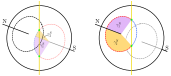
\includegraphics[width=0.7\linewidth]{gamma_limits.pdf}
  \caption{Diagrams of Earth at its perihelion (left) and aphelion (right) from a top-down perspective
    of the ecliptic plane with the north pole pointing out of the page. The two dashed
    circles in each diagram lie at latitudes $\varphi$ and $-\varphi$ in the
    northern and southern hemispheres respectively. The yellow line separates
    the day and night on Earth, with the sun illuminating the red sections of the
    circles. The longitudinal boundaries for these sections (green) are
    measured from the Earth centred Earth-fixed $x$-axis.}
  \label{fig:gamma_limits}
\end{figure}

If we now compare this to the insolation over $\psi$ on the perihelion side of
the orbit, occurring at angle $\theta_{\mathrm{A}}+\pi$, we will see that the
opposite hemisphere, at latitude $-\varphi$, receives the same insolation. 
Figure \ref{fig:gamma_limits} shows that, regardless of precession, the
longitudinal range over which irradiance reaches a given latitude is the same
on the opposite side of the orbit at the opposite latitude on Earth. Since
longitude is always measured from the Earth centred Earth-fixed $x$-axis, the
southern limits are offset from the northern limits by $\pi$, hence we can define
the southern limits as $\gamma_1^{\mathrm{S}}=\pi-\gamma_1^{\mathrm{N}}$ and
$\gamma_2^{\mathrm{S}}=\pi-\gamma_2^{\mathrm{N}}$.

Following the same steps as before but for the perihelion
side of the orbit, the insolation at latitude $-\varphi$ is
\[
\begin{split}
  Q_{\mathrm{P}} &=\frac{KP}{8\pi^2 a b}\int_{\theta_{\mathrm{A}}+\pi-\frac{\psi}{2}}^{
  \theta_{\mathrm{A}}+\pi+\frac{\psi}{2}}\int_{\pi-\gamma_1^{\mathrm{N}}}^{\pi-\gamma_2^{\mathrm{N}}}S(\theta,
  \beta,\rho,-\varphi,\gamma)\,\mathrm{d}\gamma \,\mathrm{d}\theta\\
  &= \frac{KP}{8\pi^2 a b}\int_{\theta_{\mathrm{A}}-\frac{\psi}{2}}^{\theta_{\mathrm{A}}+\frac{\psi}{2}}
  \int_{\gamma_1^{\mathrm{N}}}^{\gamma_2^{\mathrm{N}}} S((\theta+\pi),\beta,\rho,-\varphi,(\pi-\gamma))\,
  \mathrm{d}\gamma \,\mathrm{d}\theta\\
  &= \frac{KP}{8\pi^2 a b}\biggl[\Bigl[(\gamma-\pi) \sin{\beta} \sin{\varphi}
  \sin(\rho - \theta) \\
  &\quad\quad\quad\quad+ (\sin{\gamma} \sin{(\rho - \theta)} \cos{\beta} -
\cos{\gamma} \cos(\rho -
\theta))\cos{\varphi}\Bigr]_{\gamma_1^{\mathrm{N}}}^{\gamma_2^{\mathrm{N}}}
\biggr]_{\theta_{\mathrm{A}}-\frac{\psi}{2}}^{\theta_{\mathrm{A}}+\frac{\psi}{2}},
\end{split}
\]
which is equivalent to (\ref{eq:north_summer_solstice}).

\section{Recap}
Beginning with the Milankovitch cycles, we examined the different frequencies
of the orbital parameters that are believed to play an important role in
Earth's glacial periods. The variation of these orbital parameters were
implemented into Budyko's energy balance model, which demonstrates the positive
feedback effect of polar icecap albedo. However they were found to make no
significant difference to the dynamics of the ice line. In reality, the dynamics of
Earth's ice line closely match the frequency of the orbital parameters,
matching the 41\,k year period of obliquity before the MPT, and the 100\,k
year period of eccentricity since. This leads us to conclude that there must be
other feedback mechanisms at play, allowing the small external forcing from
orbital parameters to play a large role in Earth's climate.

To better understand the formulation of the Budyko model, we derived an
expression for average insolation from first principles. Through this
expression we were able to conclude that the average yearly insolation is
always symmetrically distributed over the north and south hemispheres. This supports the decision in the
Budyko model to consider just the northern hemisphere. The individual effects
of eccentricity and obliquity on the yearly average insolation were
established, as well as the independence from precession. Eccentricity was
found to scale the magnitude of the yearly average curve, whilst obliquity
altered the shape, without affecting the global average insolation for the
year. This was then compared with the insolation term from the Budyko model,
which was improved by Widiasih to include dependence on the orbital parameters.
The approximation was within 2\% of the actual yearly insolation, suggesting
that this component of the Budyko model is suitably accurate.
\bibliographystyle{ieeetr}
\bibliography{refs}
\end{document}
